\section{Introduction}

\epigraphwidth=0.3\textwidth
\epigraph{\emph{My products are my students.}}{---David Huffman}

\begin{wrapfigure}{r}{0.2\textwidth}
  \begin{center}
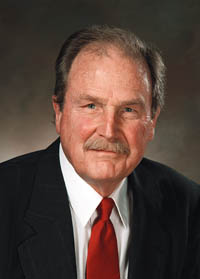
\includegraphics[width=0.15\textwidth]{images/huffman.jpg}
\centerline{\small David A. Huffman}
  \end{center}
\end{wrapfigure}

When David Huffman was a graduate student in a class at MIT, the
professor gave the class an unsolved problem: How to construct an
optimal static encoding of information. The young Huffman came back
a few days later with his solution, and that solution changed the
world. Data compression is now used in all aspects of communication.
David Huffman joined the faculty of MIT in 1953, and in 1967 he
joined the faculty of University of California, Santa Cruz as one
of its earliest members and helped to found its Computer Science
Department, where he served as chairman from 1970 to 1973. He retired
in 1994, and passed away in 1999.

The key idea is called \emph{entropy}, originally defined by Claude Shannon in
1948. Entropy is a measure of the amount of information in a, say, set of
symbols. If we define $I(x) = \log_2 \Pr[x]$ to be the information content of
a symbol, then the entropy of the set $X=\{x_1, \ldots, x_n \}$ is
$$
H(X) = \sum_{i=1}^n \Pr[x_i] I(x_i) = - \sum_{i=1}^n \Pr[x_i] \log_2 \Pr[x_i].
$$
It should be easy to see that the optimal \emph{static} encoding will assign
the least number of \emph{bits} to the most common symbol, and the greatest
number of bits to the least common symbol.
